\documentclass{homework}
\usepackage{bussproofs}
\EnableBpAbbreviations
\usepackage{ctex,hyperref,float,algorithm,algorithmic}
\hypersetup{hidelinks,
	colorlinks=true,
	allcolors=blue,
	pdfstartview=Fit,
	breaklinks=true
}

\name{熊泽恩} % Replace (Student Name) with your name.
\id{2022011223}
\term{2024 Spring}
\course{Introduction to Theoretical Computer Science}
\hwnum{7}

%\hwname{(Name)}          % Uncomment and replace (Name) with the type of the
                          % homework (e.g, Assignment, Problem Set, etc.) if you
                          % don't want the document to be labeled as "Homework."
%\problemname{(Name)}     % Uncomment and replace (Name) with the desired label
                          % for problems created with the problem environment.
%\solutionname{(Name)}    % Uncomment and replace (Name) with the desired label
                          % for solutions created with the solution environment.

% Load any other packages you need here.

\begin{document}

\begin{problem}
  Let $\problemsty{D\text{-}SAT}$ be the problem of deciding if a CNF formula
  $\varphi$ has at least two satisfying assignment.
  Prove that $\problemsty{D\text{-}SAT}$ is $\NPC$.
\end{problem}

\begin{solution}

  Firstly, it is easy to see that $\problemsty{D\text{-}SAT}$ is in $\NP$.
  Given two different sets of assignments, we can verify if they are both
  satisfying assignments in polynomial time.

  Now we prove that $\problemsty{SAT} \le_P\problemsty{D\text{-}SAT}$.
  Given a CNF formula $\varphi$, we construct a new CNF formula
  $\varphi' = \varphi \lor \varphi^{-}$.
  Here, if $\varphi=\varphi(x_1, x_2, \ldots, x_n)$,
  then $\varphi^{-} = \varphi(\neg x_1, \neg x_2, \ldots, \neg x_n)$.
  If $\varphi \in \problemsty{SAT}$, then $\varphi'$ has at least two
  satisfying assignments, namely, the satisfying assignments of $\varphi$ and
  the satisfying assignments of $\varphi^{-}$.
  If $\varphi \notin \problemsty{SAT}$,
  then $\varphi^{-}$ has no satisfying assignments either,
  so $\varphi'$ has no satisfying assignments.
  Therefore, we have constructed a computable function
  $f: \varphi \mapsto (\varphi \lor \varphi^{-})$ such that
  $\varphi \in \problemsty{SAT}$ if and only if $f(\varphi) \in \problemsty{D\text{-}SAT}$.
  Thus, have shown that $\problemsty{SAT} \le_P\problemsty{D\text{-}SAT}$.

  Since $\problemsty{SAT}$ is $\NPC$, we have $\problemsty{D\text{-}SAT}$ is $\NPC$.

\end{solution}

\begin{problem}
  A coloring of a graph is an assignment of colors to vertices in a graph so
  that no adjacent vertices have the same color.
  Let $\THREECOL$ be the problem of deciding if a given graph $G$ has a coloring
  using three colors.
  \begin{parts}
    \part\label{a}
    We will consider two graph gadgets.
    First, the triangle graph enforces that the vertices have different colors
    and you can use two of the colors $\mathrm{T}$ and $\mathrm{F}$ to encode
    true and false.
    Second, the OR gadget given in the following graph implements the logical OR
    operation.
    Prove that the OR gadget has the property that (1) if both vertices $x$ and
    $y$ have color $\mathrm{F}$, then so is the vertex labeled by $x \lor y$;
    and (2) if one of them has color $\mathrm{T}$, then it is possible to assign
    $\mathrm{T}$ to the vertex $x \lor y$ in the gadget.

    \begin{figure}[htb!]
      \centering
      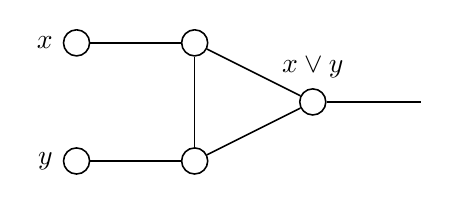
\begin{tikzpicture}[line width=.2mm]
        \pgfmathsetmacro{\h}{1.5}
        \pgfmathsetmacro{\w}{1.5}

        \node[draw,circle,label=left:{$y$}] (A0) at (0,0) {};
        \node[draw,circle,label=left:{$x$}] (B0) at (0,\h) {};

        \node[draw,circle] (A1) at (\w,0) {};
        \node[draw,circle] (B1) at (\w,\h) {};

        \node[draw,circle,label=above:{$x \lor y$}] (C) at (\w * 2,\h * .5) {};
        \node[] (D) at (\w * 3,\h * .5) {};

        \draw (A0) -- (A1);
        \draw (B0) -- (B1);
        \draw (A1) -- (B1);
        \draw (A1) -- (C);
        \draw (B1) -- (C);
        \draw (C) -- (D);
      \end{tikzpicture}
    \end{figure}

    \part\label{b}
    Use the above graph gadgets to prove that $\THREECOL$ is $\NPC$.
  \end{parts}
\end{problem}

\begin{solution}

  \ref{a}
  Let the third color be $\mathrm{U}$.

  (1) There are only two cases, and in either case,
    the vertex $x \lor y$ can only be colored $\mathrm{F}$.

  \begin{figure}[H]
    \centering
    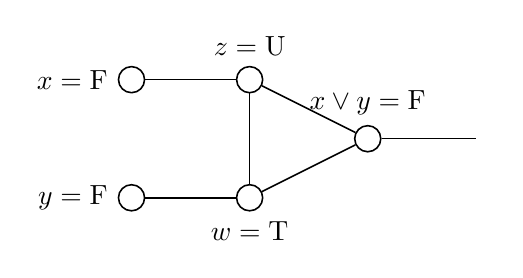
\begin{tikzpicture}[line width=.2mm]
      \pgfmathsetmacro{\h}{1.5}
      \pgfmathsetmacro{\w}{1.5}

      \node[draw,circle,label=left:{$y = \mathrm{F}$}] (A0) at (0,0) {};
      \node[draw,circle,label=left:{$x = \mathrm{F}$}] (B0) at (0,\h) {};

      \node[draw,circle,label=below:{$w = \mathrm{T}$}] (A1) at (\w,0) {};
      \node[draw,circle,label=above:{$z = \mathrm{U}$}] (B1) at (\w,\h) {};

      \node[draw,circle,label=above:{$x \lor y = \mathrm{F}$}] (C) at (\w * 2,\h * .5) {};
      \node[] (D) at (\w * 3,\h * .5) {};

      \draw (A0) -- (A1);
      \draw (B0) -- (B1);
      \draw (A1) -- (B1);
      \draw (A1) -- (C);
      \draw (B1) -- (C);
      \draw (C) -- (D);
    \end{tikzpicture}
  \end{figure}

  \begin{figure}[H]
    \centering
    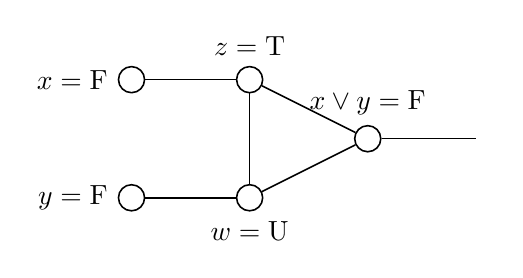
\begin{tikzpicture}[line width=.2mm]
      \pgfmathsetmacro{\h}{1.5}
      \pgfmathsetmacro{\w}{1.5}

      \node[draw,circle,label=left:{$y = \mathrm{F}$}] (A0) at (0,0) {};
      \node[draw,circle,label=left:{$x = \mathrm{F}$}] (B0) at (0,\h) {};

      \node[draw,circle,label=below:{$w = \mathrm{U}$}] (A1) at (\w,0) {};
      \node[draw,circle,label=above:{$z = \mathrm{T}$}] (B1) at (\w,\h) {};

      \node[draw,circle,label=above:{$x \lor y = \mathrm{F}$}] (C) at (\w * 2,\h * .5) {};
      \node[] (D) at (\w * 3,\h * .5) {};

      \draw (A0) -- (A1);
      \draw (B0) -- (B1);
      \draw (A1) -- (B1);
      \draw (A1) -- (C);
      \draw (B1) -- (C);
      \draw (C) -- (D);
    \end{tikzpicture}
  \end{figure}

  (2) There are two cases, and in either case,
    the vertex $x \lor y$ can be colored $\mathrm{T}$.

  \begin{figure}[H]
    \centering
    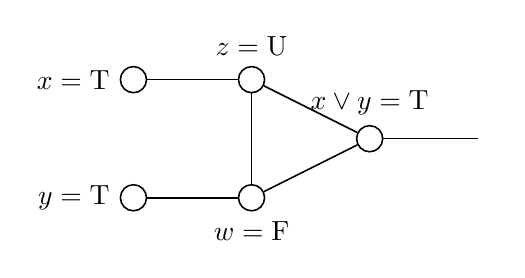
\begin{tikzpicture}[line width=.2mm]
      \pgfmathsetmacro{\h}{1.5}
      \pgfmathsetmacro{\w}{1.5}

      \node[draw,circle,label=left:{$y = \mathrm{T}$}] (A0) at (0,0) {};
      \node[draw,circle,label=left:{$x = \mathrm{T}$}] (B0) at (0,\h) {};

      \node[draw,circle,label=below:{$w = \mathrm{F}$}] (A1) at (\w,0) {};
      \node[draw,circle,label=above:{$z = \mathrm{U}$}] (B1) at (\w,\h) {};

      \node[draw,circle,label=above:{$x \lor y = \mathrm{T}$}] (C) at (\w * 2,\h * .5) {};
      \node[] (D) at (\w * 3,\h * .5) {};

      \draw (A0) -- (A1);
      \draw (B0) -- (B1);
      \draw (A1) -- (B1);
      \draw (A1) -- (C);
      \draw (B1) -- (C);
      \draw (C) -- (D);
    \end{tikzpicture}
  \end{figure}

  \begin{figure}[H]
    \centering
    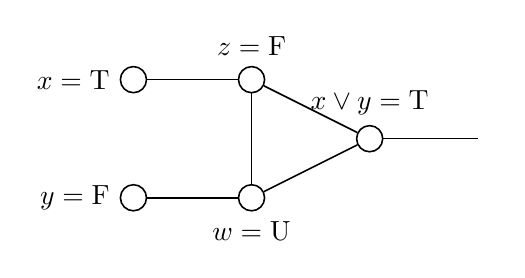
\begin{tikzpicture}[line width=.2mm]
      \pgfmathsetmacro{\h}{1.5}
      \pgfmathsetmacro{\w}{1.5}

      \node[draw,circle,label=left:{$y = \mathrm{F}$}] (A0) at (0,0) {};
      \node[draw,circle,label=left:{$x = \mathrm{T}$}] (B0) at (0,\h) {};

      \node[draw,circle,label=below:{$w = \mathrm{U}$}] (A1) at (\w,0) {};
      \node[draw,circle,label=above:{$z = \mathrm{F}$}] (B1) at (\w,\h) {};

      \node[draw,circle,label=above:{$x \lor y = \mathrm{T}$}] (C) at (\w * 2,\h * .5) {};
      \node[] (D) at (\w * 3,\h * .5) {};

      \draw (A0) -- (A1);
      \draw (B0) -- (B1);
      \draw (A1) -- (B1);
      \draw (A1) -- (C);
      \draw (B1) -- (C);
      \draw (C) -- (D);
    \end{tikzpicture}
  \end{figure}

  \ref{b}
  Firstly, it is easy to see that $\THREECOL$ is in $\NP$.
  Given a coloring of the vertices,
  we can verify if it is a valid coloring in polynomial time.

  Now we prove that $\THREESAT \le_P\THREECOL$.
  Given a $\THREESAT$ instance $\varphi$ with variables $x_1, x_2, \ldots, x_n$
  and clauses $C_1, C_2, \ldots, C_m$,
  we construct a graph $G$ as follows.

  First of all, we can assign two vertices
  to have color $\mathrm{F}$ and $\mathrm{U}$ respectively.

  \begin{figure}[H]
    \centering
    
\begin{tikzpicture}[line width=.2mm]
      \pgfmathsetmacro{\h}{1.5}
      \pgfmathsetmacro{\w}{1.5}

      \node[draw,circle,label=left:{$\mathrm{F}$}] (A0) at (0,0) {};
      \node[draw,circle,label=right:{$\mathrm{U}$}] (B0) at (\w,0) {};

      \draw (A0) -- (B0);
    \end{tikzpicture}
  \end{figure}

  Suppose $C_i = l_{i1} \lor l_{i2} \lor l_{i3}$, where $l_{ij}$ is a literal,
  meaning that either $l_{ij} = x_k$ or $l_{ij} = \neg x_k$.
  We can construct a gadget $C_i$ for each clause $C_i$ as follows.

  \begin{figure}[H]
    \centering
    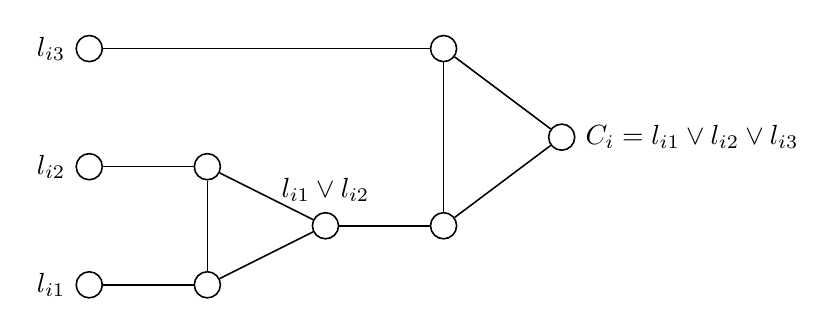
\begin{tikzpicture}[line width=.2mm]
      \pgfmathsetmacro{\h}{1.5}
      \pgfmathsetmacro{\w}{1.5}

      \node[draw,circle,label=left:{$l_{i1}$}] (A0) at (0,0) {};
      \node[draw,circle,label=left:{$l_{i2}$}] (B0) at (0,\h) {};
      \node[draw,circle,label=left:{$l_{i3}$}] (C0) at (0,\h * 2) {};

      \node[draw,circle] (A1) at (\w,0) {};
      \node[draw,circle] (B1) at (\w,\h) {};
      \node[draw,circle] (C1) at (\w * 3,\h * 2) {};

      \node[draw,circle,label=above:{$l_{i1} \lor l_{i2}$}] (C) at (\w * 2,\h * .5) {};
      \node[draw,circle] (D1) at (\w * 3,\h * .5) {};

      \node[draw,circle,label=right:{$C_i = l_{i1} \lor l_{i2} \lor l_{i3}$}] (E) at (\w * 4,\h * 1.25) {};

      \draw (A0) -- (A1);
      \draw (B0) -- (B1);
      \draw (C0) -- (C1);
      \draw (A1) -- (B1);
      \draw (A1) -- (C);
      \draw (B1) -- (C);
      \draw (C) -- (D1);
      \draw (C1) -- (D1);
      \draw (C1) -- (E);
      \draw (D1) -- (E);
    \end{tikzpicture}
  \end{figure}

  Then we connect all the gadgets $C_i$ to enforce that all of them are true.

  \begin{figure}[H]
    \centering
    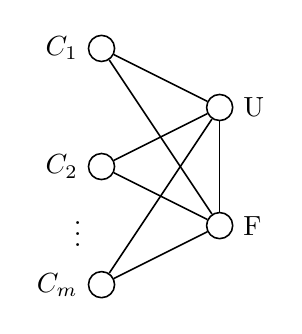
\begin{tikzpicture}[line width=.2mm]
      \pgfmathsetmacro{\h}{1.5}
      \pgfmathsetmacro{\w}{1.5}

      \node[draw,circle,label=left:{$C_m$}] (A0) at (0,0) {};
      \node[label=left:{$\vdots$}] (X) at (0,\h * 0.5) {};
      \node[draw,circle,label=left:{$C_2$}] (B0) at (0,\h) {};
      \node[draw,circle,label=left:{$C_1$}] (C0) at (0,\h * 2) {};

      \node[draw,circle,label=right:{$\mathrm{F}$}] (A1) at (\w,\h * .5) {};
      \node[draw,circle,label=right:{$\mathrm{U}$}] (B1) at (\w,\h * 1.5) {};

      \draw (A0) -- (A1);
      \draw (B0) -- (A1);
      \draw (C0) -- (A1);
      \draw (A0) -- (B1);
      \draw (B0) -- (B1);
      \draw (C0) -- (B1);
      \draw (A1) -- (B1);
    \end{tikzpicture}
  \end{figure}

  Finally, we connect all the variables to enforce that all of them are colored.

  \begin{figure}[H]
    \centering
    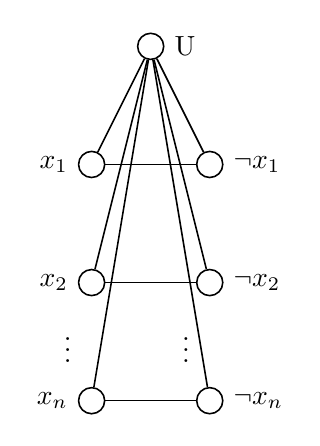
\begin{tikzpicture}[line width=.2mm]
      \pgfmathsetmacro{\h}{1.5}
      \pgfmathsetmacro{\w}{1.5}

      \node[draw,circle,label=left:{$x_n$}] (A0) at (0,0) {};
      \node[label=left:{$\vdots$}] (D) at (0,\h * 0.5) {};
      \node[draw,circle,label=left:{$x_2$}] (B0) at (0,\h) {};
      \node[draw,circle,label=left:{$x_1$}] (C0) at (0,\h * 2) {};

      \node[draw,circle,label=right:{$\neg x_n$}] (A1) at (\w,0) {};
      \node[label=left:{$\vdots$}] (D) at (\w,\h * 0.5) {};
      \node[draw,circle,label=right:{$\neg x_2$}] (B1) at (\w,\h) {};
      \node[draw,circle,label=right:{$\neg x_1$}] (C1) at (\w,\h * 2) {};

      \node[draw,circle,label=right:{$\mathrm{U}$}] (Y) at (\w * .5,\h * 3) {};

      \draw (A0) -- (A1);
      \draw (B0) -- (B1);
      \draw (C0) -- (C1);
      \draw (A0) -- (Y);
      \draw (A1) -- (Y);
      \draw (B0) -- (Y);
      \draw (B1) -- (Y);
      \draw (C0) -- (Y);
      \draw (C1) -- (Y);
    \end{tikzpicture}
  \end{figure}

  If $\varphi$ is satisfiable, then the graph $G$ has a three-coloring.
  If $\varphi$ is not satisfiable, then the graph $G$ does not have a three-coloring.
  Therefore, we have constructed a computable function
  $f: \varphi \mapsto G$ such that
  $\varphi \in \THREESAT$ if and only if $f(\varphi) \in \THREECOL$.
  Thus, have shown that $\THREESAT \le_P\THREECOL$.

\end{solution}

\begin{problem}
  Write a complete proof for the Claim 1 in the proof of Ladner's theorem
  discussed in class.
  That is, show that both $Z(n)$ and $n^{Z(n)}$ are computable in time
  polynomial in $n$.
  The definition of $Z(n)$ is given in the lecture notes.
\end{problem}

\begin{solution}

  Definition of $Z$: Enumerate all TMs $M_1, M_2, \cdots$. Define $Z(1) = 1$.
  Suppose $Z(n-1) = i$. If for all $x$ of length at most $\log n$,
  $M_i$ computes $\SAT_Z(x)$, $Z(n) = i$. Otherwise, define $Z(n) = i+1$.

  Firstly, we will show that $Z(n)$ is computable in time polynomial in $n$.
  We will prove this by induction on $n$.
  It is apparent that $Z(1)$ could be computed in constant time,
  thus is polynomial in $n$.
  Suppose that $Z(n-1)$ is computable in time polynomial in $n-1$,
  which is also polynomial in $n$.
  Now let's consider $Z(n)$.
  Since we can compute $Z(n - 1)$ in polynomial time,
  we can enumerate all TMs $M_1, M_2, \cdots, M_{Z(n-1)}$, and get $M_{Z(n-1)}$.
  Then we can compute $\SAT_Z(x)$ for all $x$ of length at most $\log n$.
  Note that the alphabet of $x$, denoted as $\Sigma$, is finite,
  so the number of $x$ of length at most $\log n$ is finite,
  which is on the order of $O(|\Sigma|^{\log n}) = O(n^{\log|\Sigma|})$,
  and can be computed in polynomial time.
  Then, we can verify if $M_{Z(n-1)}$ computes $\SAT_Z(x)$ for all $x$ of length at most $\log n$.
  Hence, we can compute $Z(n)$ in polynomial time.

  Secondly, we will show that $n^{Z(n)}$ is computable in time polynomial in $n$.
  Since $Z(n)$ is represented in binary format,
  the length of $Z(n)$ is on the order of $O(\log Z(n))$.
  Each multiplication can be done in polynomial time in $n$,
  and we need to multiply $n$ by itself $Z(n)$ times,
  where $Z(n) = O(\log\log n)$.
  Therefore, $n^{Z(n)}$ is computable in time polynomial in $n$.

  Therefore, both $Z(n)$ and $n^{Z(n)}$ are computable in time polynomial in $n$.

\end{solution}

\end{document}
